\subsection{Feature Extraction Pipeline}
\label{subsec:feature_extraction}
Following the preprocessing of raw signal arrays, the pipeline transits into a highly dimensional analytic space via the multi-modal feature extraction engine. The core philosophy of this sub-architecture embraces the complexity of neuronal non-stationarity—instead of deriving purely statistical averages, a unified framework synchronously evaluates temporal dynamics, spectral geometries, networked connectivity, and non-linear complexity. Implemented via \texttt{extraction.py} and its subordinate modules within \texttt{pipeline/src/feature\_extraction}, this system dynamically batches processed FIF and MNE structures to form flattened machine-learning-ready tensors.

\begin{figure}[htpb]
    \centering
    \resizebox{\textwidth}{!}{
    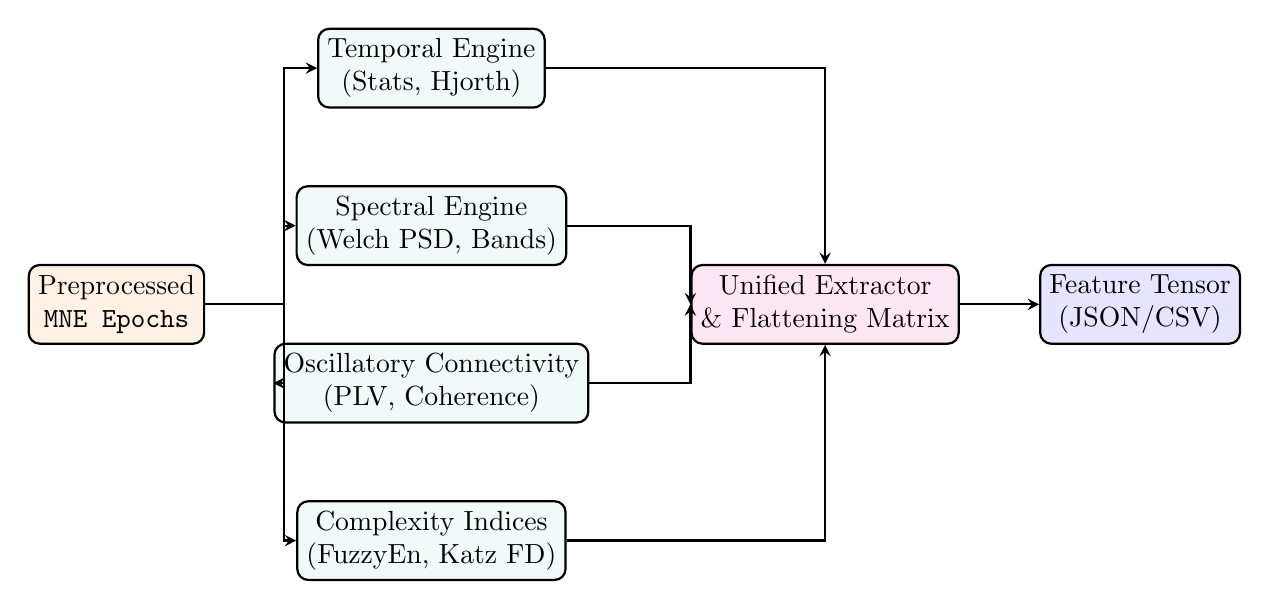
\begin{tikzpicture}[
        box/.style={draw, rectangle, rounded corners, align=center, minimum height=1cm, fill=teal!5, thick},
        arrow/.style={->, thick, -stealth}
    ]
        \node[box, fill=orange!10] (input) at (0, 0) {Preprocessed \\ \texttt{MNE Epochs}};
        
        \node[box] (time) at (4, 3) {Temporal Engine \\ (Stats, Hjorth)};
        \node[box] (freq) at (4, 1) {Spectral Engine \\ (Welch PSD, Bands)};
        \node[box] (conn) at (4, -1) {Oscillatory Connectivity \\ (PLV, Coherence)};
        \node[box] (fuzzy) at (4, -3) {Complexity Indices \\ (FuzzyEn, Katz FD)};
        
        \node[box, fill=magenta!10] (agg) at (9, 0) {Unified Extractor \\ \& Flattening Matrix};
        \node[box, fill=blue!10] (output) at (13, 0) {Feature Tensor \\ (JSON/CSV)};

        \draw[arrow] (input.east) -- ++(1,0) |- (time.west);
        \draw[arrow] (input.east) -- ++(1,0) |- (freq.west);
        \draw[arrow] (input.east) -- ++(1,0) |- (conn.west);
        \draw[arrow] (input.east) -- ++(1,0) |- (fuzzy.west);
        
        \draw[arrow] (time.east) -| (agg.north);
        \draw[arrow] (freq.east) -| (agg.west);
        \draw[arrow] (conn.east) -| (agg.west);
        \draw[arrow] (fuzzy.east) -| (agg.south);
        \draw[arrow] (agg.east) -- (output.west);
    \end{tikzpicture}
    }
    \caption{Functional schematic of the feature extraction architecture, illustrating parallel computation across four distinct signal domains.}
    \label{fig:feat_extraction_process}
\end{figure}

\subsubsection{Temporal Dynamic Parameterization}
The temporal sub-module prioritizes both descriptive statistics and transient shift recognition, acknowledging that early-stage cognitive decline heavily disturbs generalized steady-state continuous amplitude \cite{jeong2004eeg}. Beyond base calculations (mean, variance, skewness, and IQR), the \texttt{time\_domain.py} explicitly computes the Hjorth Parameters: Activity, Mobility, and Complexity.

The derivation of Hjorth Mobility $M(x)$ essentially defines the root-mean-square frequency, standardizing the signal's first derivative against the base amplitude:
\begin{equation}
    M(x) = \sqrt{\frac{\text{var}(x')}{\text{var}(x)}}
\end{equation}
where $x'$ denotes the instantaneous temporal derivative of the EEG channel vector $x$. 
Correspondingly, Hjorth Complexity $C(x)$ acts as a soft measure of bandwidth, quantifying the deviation of the signal's spectral slope from a pure sinusoid. The inclusion of Hjorth limits is an evidence-backed requirement; literature demonstrates that an increase in temporal complexity directly tracks the pathological pseudo-randomization of neural firing typical in the transition from MCI (Mild Cognitive Impairment) to clinical Alzheimer's \cite{cassani2020review}.

\subsubsection{Spectral Profiling and Energy Ratios}
Operated by \texttt{frequency\_domain.py}, the spectral feature mapper executes localized Welch's periodogram sweeps on channel segments. Instead of naive Fast Fourier Transforms (FFT), Welch's method computes power spectral density (PSD) with overlapping Hann windows (typically utilizing a 2-second resolution with 50\% overlap to ensure the retention of stationary micro-states).

\begin{equation}
    P_{Welch}(f) = \frac{1}{K} \sum_{k=1}^{K} P_k(f)
\end{equation}

Power indices are segregated into classical bands: $\delta$ (0.5--4 Hz), $\theta$ (4--8 Hz), $\alpha$ (8--13 Hz), $\beta$ (13--30 Hz), and $\gamma$ (30--45 Hz). As validated by the 40Hz biomarker paradigm \cite{martorell2019gamma}, absolute and relative regional $\gamma$ band concentrations—specifically computed to mitigate baseline drift—are fundamental indices exported into the unified JSON metadata structures.

\subsubsection{Phase-Synchronous Connectivity Mapping}
The degeneration of cholinergic pathways in prolonged Alzheimer's causes localized network dysconnection, transforming the brain from a small-world topology into a fragmented matrix. To natively track this, the \texttt{connectivity.py} domain employs dense correlative computations yielding $N \times N$ adjacency matrices (where $N$ defines topologic sensor count).

The principal metric extracted is the robust Phase Locking Value (PLV), filtering out arbitrary amplitude modulations and directly isolating cross-channel temporal lag synchronization:
\begin{equation}
    \text{PLV}_{x,y} = \left| \frac{1}{T} \sum_{t=1}^{T} e^{i(\phi_x(t) - \phi_y(t))} \right|
\end{equation}
Operating over specific frequencies, specifically the high $\beta$ and steady-state 40Hz $\gamma$ arrays, the system computes the global mean clustering coefficient across the upper triangular matrix to synthesize the matrix into a singular numerical input required for standard algorithmic ingestion. 

\subsubsection{Non-Linear and Fuzzy Feature Abstraction}
In tandem with linear metrics, the \texttt{fuzzy\_features.py} process calculates geometric indices of waveform fractality and embedded chaos. Specifically, the \textbf{Katz Fractal Dimension} captures signal jitter across discrete sampling frames, while \textbf{Fuzzy Entropy (FuzzyEn)} models stochastic phase-space irregularities without generating infinite gradient constraints common to classical Sample Entropy \cite{stam2007graph}. 
FuzzyEn is defined via the Chebyshev continuous distance constraint $D_{i,j}^m$ between embedded vectors, applying a negative exponential fuzzy membership function constraint:
\begin{equation}
    \mu(D_{i,j}^m, r, n) = \exp \left(-\frac{(D_{i,j}^m)^n}{r} \right)
\end{equation}
This bounds structural unpredictability strictly between $0 \to 1$, offering an unprecedented, standardized representation of pathological complexity to feed into neural weighting models.

\subsubsection{Algorithmic Dimensional Consolidation}
Once asynchronous extraction scripts complete execution, \texttt{extraction.py} aggregates overlapping output tensors, filtering undefined geometries (NaN, infinite limits). Recognizing the constraints of classical machine learning engines, the hierarchical tensor dictionary is dynamically recursively unwrapped into a stable two-dimensional CSV file (Samples $\times$ Parameters), ensuring deterministic matrix multiplication capability in downstream prediction stages.
